\documentclass[12pt,a4paper]{article}

\usepackage[utf8]{inputenc}
\usepackage[T1]{fontenc}
\usepackage[polish]{babel}
\usepackage{geometry}
\usepackage{graphicx}
\usepackage{booktabs}
\usepackage{amsmath}
\usepackage{float}
\usepackage{hyperref}
\usepackage{caption}
\usepackage{subcaption}

\geometry{margin=2.5cm}
\hypersetup{
    colorlinks=true,
    linkcolor=black,
    urlcolor=blue
}

\title{Porownanie algorytmow scieniania odciskow palcow}
\author{Biometria -- projekt 3}
\date{\today}

\begin{document}

\maketitle

\section{Cel i zakres}

Celem projektu bylo przygotowanie programu do porownania algorytmow scieniania w odniesieniu do obrazow odciskow palcow. Zrealizowane wymagania:
\begin{itemize}
    \item implementacja trzech algorytmow scieniania: szkieletyzacji morfologicznej, K3M oraz KMM,
    \item dodatkowe operacje poprawiajace ciaglosc linii papilarnych,
    \item lokalizacja minucji (zakonczenia i bifurkacje),
    \item raport z porownaniem wynikow i wizualizacjami.
\end{itemize}

\section{Instrukcja uzytkownika}

\textbf{Instalacja:}
\begin{enumerate}
    \item \texttt{pip install -r requirements.txt}
\end{enumerate}

\textbf{Uruchomienie aplikacji:}
\begin{enumerate}
    \item \texttt{python app.py}
\end{enumerate}

GUI pozwala zaladowac obrazy demo, dobrac parametry oraz wyeksportowac dashboard i wyniki w formacie JSON.

\section{Struktura rozwiazania i technologie}

Najwazniejsze pliki projektu:
\begin{itemize}
    \item \texttt{fingerprint\_processor.py} -- pipeline przetwarzania, scienianie i minucje,
    \item \texttt{app.py} -- GUI w \texttt{tkinter} z podgladem etapow oraz eksportem wynikow,
    \item \texttt{requirements.txt} -- zaleznosci.
\end{itemize}

Technologie: Python 3.x, biblioteka Pillow do IO i renderingu oraz \texttt{tkinter} do interfejsu graficznego.

\section{Pipeline przetwarzania}

Pipeline sklada sie z nastepujacych krokow:
\begin{enumerate}
    \item Wczytanie obrazu i wzmocnienie kontrastu (stretching percentylowy).
    \item Binaryzacja: Otsu lub adaptacyjna Sauvola (tryb \texttt{auto}).
    \item (Opcjonalnie) maska obszaru odcisku oparta o lokalne odchylenie standardowe.
    \item Czyszczenie morfologiczne (domkniecie i otwarcie).
    \item Scienianie: morfologiczne, K3M oraz KMM.
    \item Postprocessing: laczenie przerw i usuwanie krotkich odnog.
    \item Detekcja minucji metoda \emph{crossing number}.
\end{enumerate}

\section{Model matematyczny i metody}

\subsection{Binaryzacja Otsu i Sauvola}

W przypadku Sauvoli wykorzystywany jest prog lokalny:
\[
T(x,y)=m(x,y)\left(1+k\left(\frac{s(x,y)}{R}-1\right)\right),
\]
gdzie \(m\) to srednia lokalna, \(s\) to odchylenie standardowe, a \(R\) to zakres dynamiczny.

W praktyce Sauvola jest mniej wrazliwa na nierownomierne oswietlenie i lokalne spadki kontrastu.
Otsu korzysta z progu globalnego, co bywa wystarczajace dla czystych skanow, ale slabiej dziala
na obrazach z cieniem lub przyslonietymi fragmentami.

\subsection{Szkieletyzacja morfologiczna}

Algorytm opiera sie na iteracyjnym erodowaniu obrazu i zbieraniu reszty po otwarciu:
\[
S = \bigcup_{k=0}^{\infty} (I_k \setminus (I_k \circ B)), \quad I_{k+1} = I_k \ominus B.
\]

Wynikiem jest szkieletyzacja o zachowanej topologii, ale wrazliwa na szum i drobne ubytki.
Bez dodatkowego postprocessingu pojawiaja sie oderwane odnogi i lokalne rozczepienia, co
zwieksza liczbe wykrywanych zakonczen.

\subsection{K3M}

K3M to algorytm sekwencyjny z wielofazowym usuwaniem pikseli konturowych. Decyzje o usunieciu pikseli podejmowane sa na podstawie wag sasiedztwa oraz tablic faz.

Algorytm wykonuje serie faz, w ktorych piksel jest usuwany tylko wtedy, gdy spelnia warunki
dotyczace wag sasiedztwa i nie narusza spojnosci. Dzieki temu szkielety sa cienkie i stabilne,
ale algorytm wymaga kilku iteracji, przez co jest wolniejszy od metod morfologicznych.

\subsection{KMM}

KMM jest algorytmem iteracyjnym, w ktorym usuwane sa piksele spelniajace warunki topologiczne i nalezace do tablicy wag usuniecia. Dodatkowo sprawdzana jest prostota punktu (simple point).

W praktyce KMM agresywniej usuwa piksele z konturu, ale kontrola prostoty punktu ogranicza
rozrywanie grzbietow. W porownaniu do K3M czesto pozostawia nieco grubszy szkieletyzowany obraz,
co widac w liczbie pikseli szkieletu.

\subsection{Detekcja minucji}

Minucje wykrywane sa za pomoca crossing number:
\[
CN = \frac{1}{2}\sum_{i=1}^{8} |p_i - p_{i+1}|,
\]
gdzie \(CN=1\) oznacza zakonczenie, a \(CN=3\) bifurkacje. Dodatkowo stosowane jest filtrowanie po minimalnym dystansie miedzy punktami.

Detekcja wykonywana jest na szkielecie po postprocessingu. W praktyce liczba minucji jest
silnie zalezna od jakosci binaryzacji i poziomu szumu w szkielecie.

\section{Parametry i ustawienia domyslne}

W eksperymentach uzyto ustawien domyslnych aplikacji:
\begin{itemize}
    \item binarizacja: \texttt{auto} (Otsu lub Sauvola),
    \item Sauvola: okno 21, \(k=0.2\), \(R=128\),
    \item maska odcisku: wylaczona,
    \item domkniecie/otwarcie: 1,
    \item laczenie przerw: 1 iteracja, \texttt{max gap}=7,
    \item pruning odnog: 1 iteracja, \texttt{max length}=4,
    \item minimalny dystans minucji: 6 px.
\end{itemize}

Parametry sa dobrane tak, aby zachowac kompromis miedzy czuloscia detekcji minucji
a stabilnoscia szkieletu. Przy wiekszej liczbie iteracji postprocessingu liczba minucji
spada, ale spada tez szczegolowosc grzbietow, co jest widoczne zwlaszcza na slabiej
jakosci skanach.

\section{Wyniki dla obrazu igor/rsmall3}

Poniżej zestawiono wyniki dla obrazu \texttt{igor/rsmall3.bmp} z pakietu demo.

\begin{table}[H]
    \centering
    \caption{Podsumowanie wynikow dla igor/rsmall3.bmp.}
    \begin{tabular}{lrrrr}
        \toprule
        Algorytm & Prog & Piksele szkieletu & Zakonczenia & Bifurkacje \\
        \midrule
        Morfologia & 141 & 5946 & 459 & 11 \\
        K3M & 141 & 5417 & 361 & 8 \\
        KMM & 141 & 10447 & 516 & 8 \\
        \bottomrule
    \end{tabular}
\end{table}

Wyniki ilosciowe pokazuja, ze KMM generuje najwiecej pikseli szkieletu oraz najwiecej minucji typu
zakonczenie. K3M daje najcienszy szkielety (najmniej pikseli), co przeklada sie na mniejsza liczbe
wykrytych minucji. Szkieletyzacja morfologiczna jest pomiedzy tymi dwoma przypadkami, ale w praktyce
czesc minucji pochodzi z lokalnych zaklocen i przerw w binarce.

W przypadku obrazu \texttt{rsmall3.bmp} liczba bifurkacji jest podobna dla K3M i KMM, co sugeruje,
ze glowne rozgalezienia zostaly zachowane, a roznice wynikaja glownie z dodatkowych odnog oraz
zakonczen generowanych przez szum.

\section{Porownanie algorytmow}

\subsection{Jakosc szkieletu}

\begin{itemize}
    \item \textbf{Morfologia} -- szybka i prosta, ale wrazliwa na ubytki w binarce; czesto generuje
    krotkie odnogi i punkty widoczne jako dodatkowe zakonczenia.
    \item \textbf{K3M} -- stabilna topologia i cienki szkieletyzowany obraz, kosztem kilku iteracji
    i wiekszego czasu obliczen; daje najmniejsza liczbe pikseli szkieletu.
    \item \textbf{KMM} -- zachowuje strukture grzbietow, ale pozostawia nieco grubszy szkieletyzowany
    obraz, co przeklada sie na wieksza liczbe wykrytych zakonczen.
\end{itemize}

\subsection{Minucje}

Wizualizacje \ref{fig:endings} i \ref{fig:bifurcations} pokazuja, ze:
\begin{itemize}
    \item liczba zakonczen jest najbardziej wrazliwa na drobne przerwy w szkielecie,
    \item bifurkacje sa bardziej stabilne i mniej zalezne od drobnych zaklocen,
    \item K3M i KMM zachowuja podobny uklad bifurkacji, ale roznia sie licznoscia zakonczen.
\end{itemize}

\section{Omowienie wynikow}

W praktyce najwazniejsza rola pipeline'u to dostarczenie czystego szkieletu. Dla badanej probki
kluczowe okazaly sie:
\begin{itemize}
    \item adaptacyjna binarizacja (Sauvola), ktora stabilizuje widocznosc grzbietow,
    \item laczenie przerw po scienianiu, ktore redukuje sztuczne zakonczenia,
    \item pruning odnog, ktory usuwa krotkie artefakty.
\end{itemize}

Na obrazie \texttt{rsmall3.bmp} K3M daje najbardziej uporzadkowany szkieletyzowany obraz, ale kosztem
utraconej drobnej struktury. KMM zachowuje wiecej szczegolow, co bywa korzystne dla analizy
minucji, ale zwieksza liczbe punktow zakonczen. Morfologia pozostaje najbardziej wrazliwa na
szum w obrazie i wymaga najsilniejszego postprocessingu.

\section{Wizualizacje}

Poniższe obrazy zostaly wygenerowane automatycznie dla \texttt{igor/rsmall3.bmp}.

\begin{figure}[H]
    \centering
    \begin{subfigure}[t]{0.49\textwidth}
        \centering
        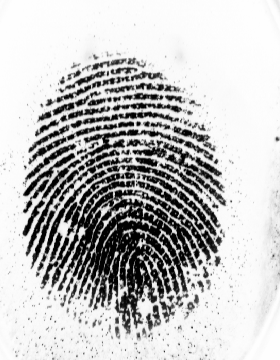
\includegraphics[width=\textwidth]{res/rsmall3_source.png}
        \caption{Oryginalny obraz wejsciowy.}
    \end{subfigure}
    \hfill
    \begin{subfigure}[t]{0.49\textwidth}
        \centering
        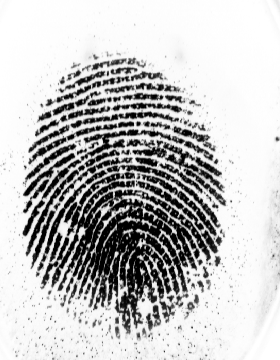
\includegraphics[width=\textwidth]{res/rsmall3_enhanced.png}
        \caption{Wzmocnienie kontrastu.}
    \end{subfigure}
    \caption{Etapy wstepnego przetwarzania.}
    \label{fig:preprocess}
\end{figure}

\begin{figure}[H]
    \centering
    \begin{subfigure}[t]{0.49\textwidth}
        \centering
        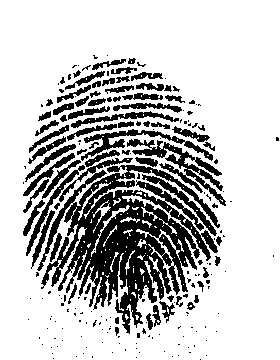
\includegraphics[width=\textwidth]{res/rsmall3_binary.png}
        \caption{Binaryzacja.}
    \end{subfigure}
    \hfill
    \begin{subfigure}[t]{0.49\textwidth}
        \centering
        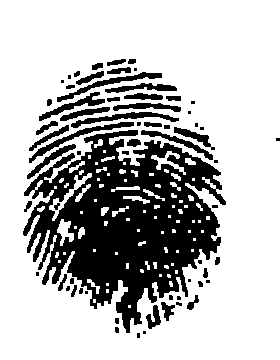
\includegraphics[width=\textwidth]{res/rsmall3_cleaned.png}
        \caption{Po czyszczeniu morfologicznym.}
    \end{subfigure}
    \caption{Binaryzacja i oczyszczanie obrazu.}
    \label{fig:binary}
\end{figure}

\begin{figure}[H]
    \centering
    \begin{subfigure}[t]{0.32\textwidth}
        \centering
        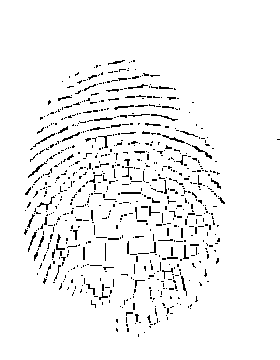
\includegraphics[width=\textwidth]{res/rsmall3_morph_raw.png}
        \caption{Szkielet morfologiczny (surowy).}
    \end{subfigure}
    \hfill
    \begin{subfigure}[t]{0.32\textwidth}
        \centering
        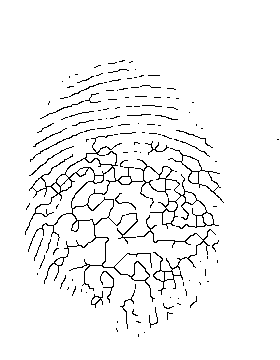
\includegraphics[width=\textwidth]{res/rsmall3_k3m_raw.png}
        \caption{K3M (surowy).}
    \end{subfigure}
    \hfill
    \begin{subfigure}[t]{0.32\textwidth}
        \centering
        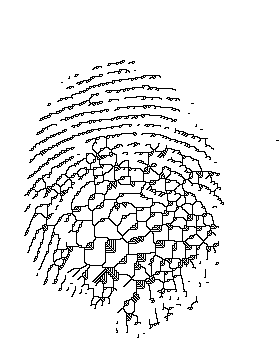
\includegraphics[width=\textwidth]{res/rsmall3_kmm_raw.png}
        \caption{KMM (surowy).}
    \end{subfigure}
    \caption{Porownanie surowych szkieletow.}
    \label{fig:raw_skeletons}
\end{figure}

\begin{figure}[H]
    \centering
    \begin{subfigure}[t]{0.32\textwidth}
        \centering
        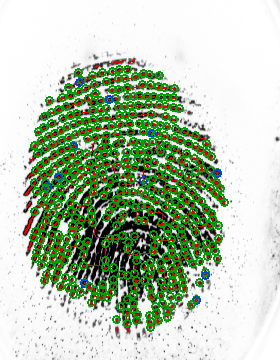
\includegraphics[width=\textwidth]{res/rsmall3_morph_all.png}
        \caption{Morfologia: wszystkie minucje.}
    \end{subfigure}
    \hfill
    \begin{subfigure}[t]{0.32\textwidth}
        \centering
        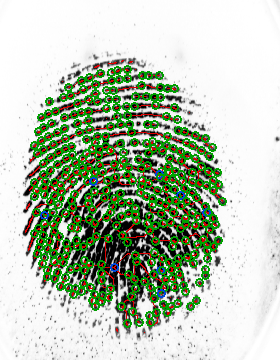
\includegraphics[width=\textwidth]{res/rsmall3_k3m_all.png}
        \caption{K3M: wszystkie minucje.}
    \end{subfigure}
    \hfill
    \begin{subfigure}[t]{0.32\textwidth}
        \centering
        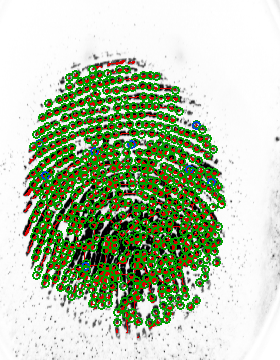
\includegraphics[width=\textwidth]{res/rsmall3_kmm_all.png}
        \caption{KMM: wszystkie minucje.}
    \end{subfigure}
    \caption{Nakladki minucji dla trzech algorytmow.}
    \label{fig:all_minutiae}
\end{figure}

\begin{figure}[H]
    \centering
    \begin{subfigure}[t]{0.32\textwidth}
        \centering
        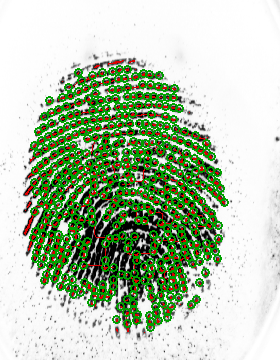
\includegraphics[width=\textwidth]{res/rsmall3_morph_endings.png}
        \caption{Morfologia: zakonczenia.}
    \end{subfigure}
    \hfill
    \begin{subfigure}[t]{0.32\textwidth}
        \centering
        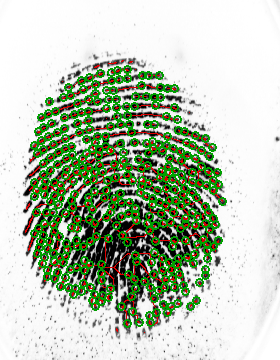
\includegraphics[width=\textwidth]{res/rsmall3_k3m_endings.png}
        \caption{K3M: zakonczenia.}
    \end{subfigure}
    \hfill
    \begin{subfigure}[t]{0.32\textwidth}
        \centering
        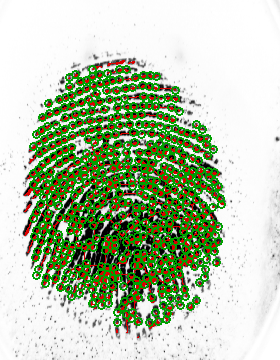
\includegraphics[width=\textwidth]{res/rsmall3_kmm_endings.png}
        \caption{KMM: zakonczenia.}
    \end{subfigure}
    \caption{Porownanie minucji typu zakonczenie.}
    \label{fig:endings}
\end{figure}

\begin{figure}[H]
    \centering
    \begin{subfigure}[t]{0.32\textwidth}
        \centering
        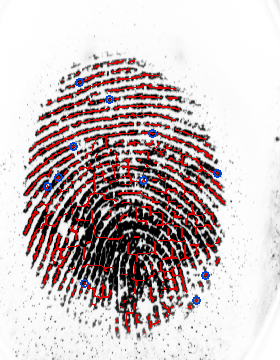
\includegraphics[width=\textwidth]{res/rsmall3_morph_bifurcations.png}
        \caption{Morfologia: bifurkacje.}
    \end{subfigure}
    \hfill
    \begin{subfigure}[t]{0.32\textwidth}
        \centering
        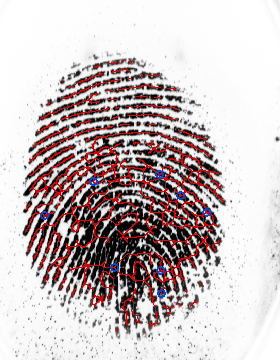
\includegraphics[width=\textwidth]{res/rsmall3_k3m_bifurcations.png}
        \caption{K3M: bifurkacje.}
    \end{subfigure}
    \hfill
    \begin{subfigure}[t]{0.32\textwidth}
        \centering
        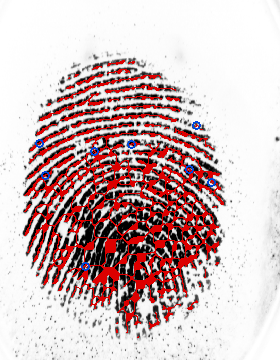
\includegraphics[width=\textwidth]{res/rsmall3_kmm_bifurcations.png}
        \caption{KMM: bifurkacje.}
    \end{subfigure}
    \caption{Porownanie minucji typu bifurkacja.}
    \label{fig:bifurcations}
\end{figure}

\section{Wnioski}

Najwazniejsze obserwacje:
\begin{itemize}
    \item Adaptacyjna binarizacja (Sauvola lub tryb \texttt{auto}) daje stabilniejsze maski dla skanow o nierownym oswietleniu.
    \item K3M i KMM generuja bardziej jednolite szkielety niz szkieletyzacja morfologiczna, szczegolnie w obszarach o slabym kontraście.
    \item Laczenie przerw i pruning odnog sa kluczowe, aby ograniczyc artefakty i falszywe minucje.
\end{itemize}

\end{document}
